% flashcards-title: Equal-value exchange between twelve ones and one ten with two ones
% flashcards-desc: On the left, twelve loose counters in rows. On the right, one outlined loop encloses ten counters and two loose counters sit beside it. A double-headed arrow labeled same quantity connects the two sides.
\documentclass[tikz]{standalone}
\usetikzlibrary{arrows.meta,patterns}

\definecolor{qraNavy}{HTML}{17324D}
\definecolor{qraBlue}{HTML}{2B6CB0}
\definecolor{qraGold}{HTML}{B7791F}
\definecolor{qraPale}{HTML}{EAF2F8}
\definecolor{qraGray}{HTML}{5C6773}

\tikzset{
  qra axis/.style={draw=qraNavy, line width=1.2pt},
  qra tick/.style={draw=qraNavy, line width=1pt},
  qra guide/.style={draw=qraGray, densely dashed, line width=0.8pt},
  qra counter/.style={circle, draw=qraNavy, fill=qraPale, line width=0.9pt, minimum size=7mm, inner sep=0pt},
  qra label/.style={font=\sffamily\bfseries, text=qraNavy},
  qra small label/.style={font=\sffamily, text=qraNavy},
}

\begin{document}
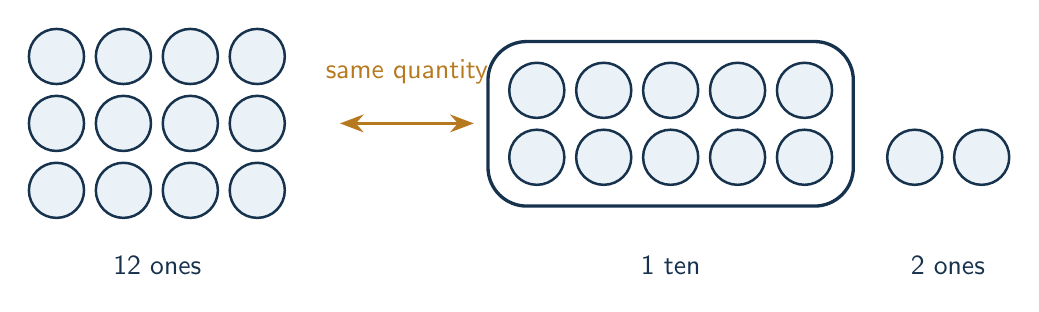
\begin{tikzpicture}
  % Left: twelve loose counters (4 columns x 3 rows)
  \foreach \i in {0,...,3} {
    \foreach \j in {0,1,2} {
      \node[qra counter] at (\i*0.85, \j*0.85) {};
    }
  }
  \node[qra small label] at (1.28,-0.95) {12 ones};

  % Double-headed arrow
  \draw[qra axis, draw=qraGold, {Stealth[length=3mm]}-{Stealth[length=3mm]}]
    (3.6,0.85) -- (5.3,0.85);
  \node[qra small label, text=qraGold] at (4.45,1.5) {same quantity};

  % Right: one loop of ten (5 x 2 grid) plus two loose counters
  \begin{scope}[xshift=6.1cm]
    \foreach \i in {0,...,4} {
      \foreach \j in {0,1} {
        \node[qra counter] at (\i*0.85, \j*0.85+0.42) {};
      }
    }
    \draw[qra axis, rounded corners=14pt] (-0.62,-0.2) rectangle (4.02,1.89);
    \node[qra small label] at (1.7,-0.95) {1 ten};

    \node[qra counter] at (4.8,0.42) {};
    \node[qra counter] at (5.65,0.42) {};
    \node[qra small label] at (5.22,-0.95) {2 ones};
  \end{scope}
\end{tikzpicture}
\end{document}
